\section{\texorpdfstring{Decision Making with Analytical Hierarchy
Process
}{Decision Making with Analytical Hierarchy Process }}\label{decision-making-with-analytical-hierarchy-process}

Making good decisions is a crucial skill at every level.---Peter Drucker

A hallmark of design is that many decisions must be made throughout the
process. Typically, there are alternative solutions to a problem from
which the best one relative to some criteria is selected. This appendix
presents the Analytical Hierarchy Process (AHP) approach to decision
making. AHP is a flexible quantitative and qualitative method that is
applicable to many problems which provides a numerical score for the
alternatives considered. Different aspects of AHP are applied throughout
the text and this appendix is structured to teach AHP via example. A
summary of AHP is provided at the conclusion of the appendix.

To apply AHP there must be a decision to be made, criteria against which
the decision is based, and a set of competing decisions from which one
must be selected. This process is encapsulated in the decision matrix
shown in Table B.1 and as such the process is sometimes referred to as
the \emph{\textbf{decision-matrix method}}. The row headings are the
criteria against which the decision is made and the column headings
represent the alternatives. The criteria can have differing levels of
importance and their relative weightings are reflected by
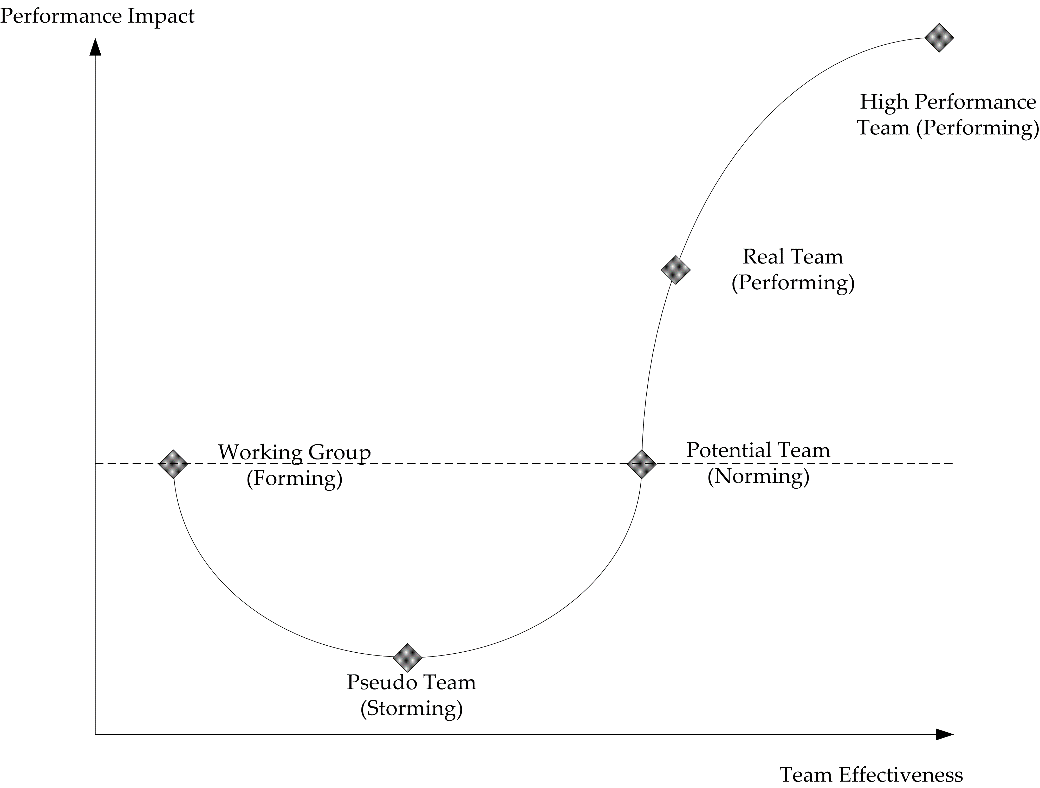
\includegraphics{Fig/media/image1.wmf} values in the matrix. The entries
in the matrix, 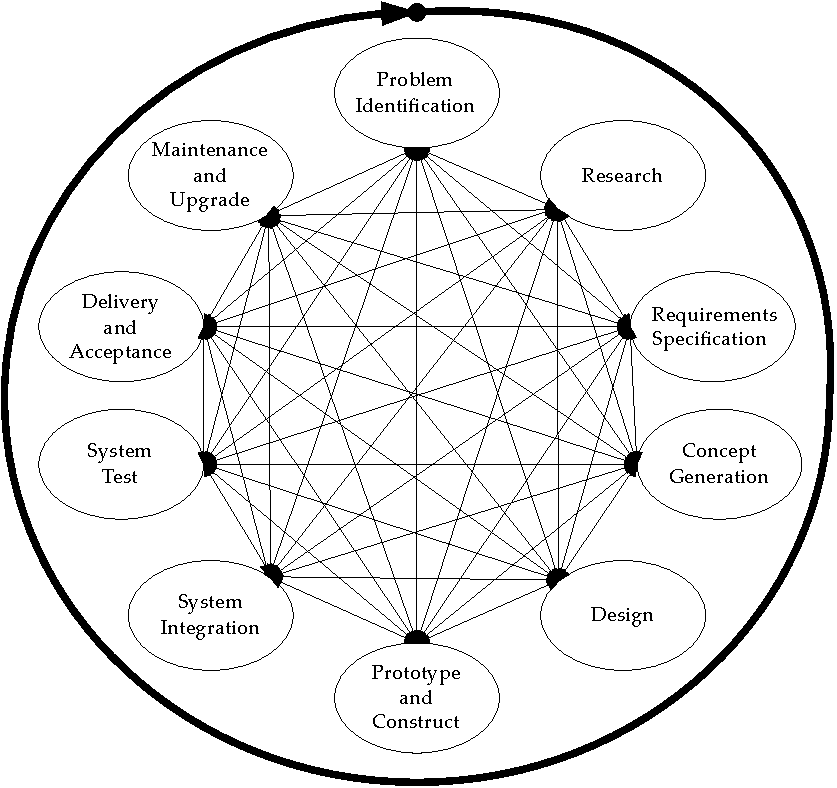
\includegraphics{Fig/media/image2.wmf}, are ratings for
each \emph{j\textsuperscript{th}} alternative relative to
\emph{i\textsuperscript{th}} criterion. Each alternative receives a
score, \emph{S\textsubscript{j}}, which is a weighted sum of the ratings
that is computed as

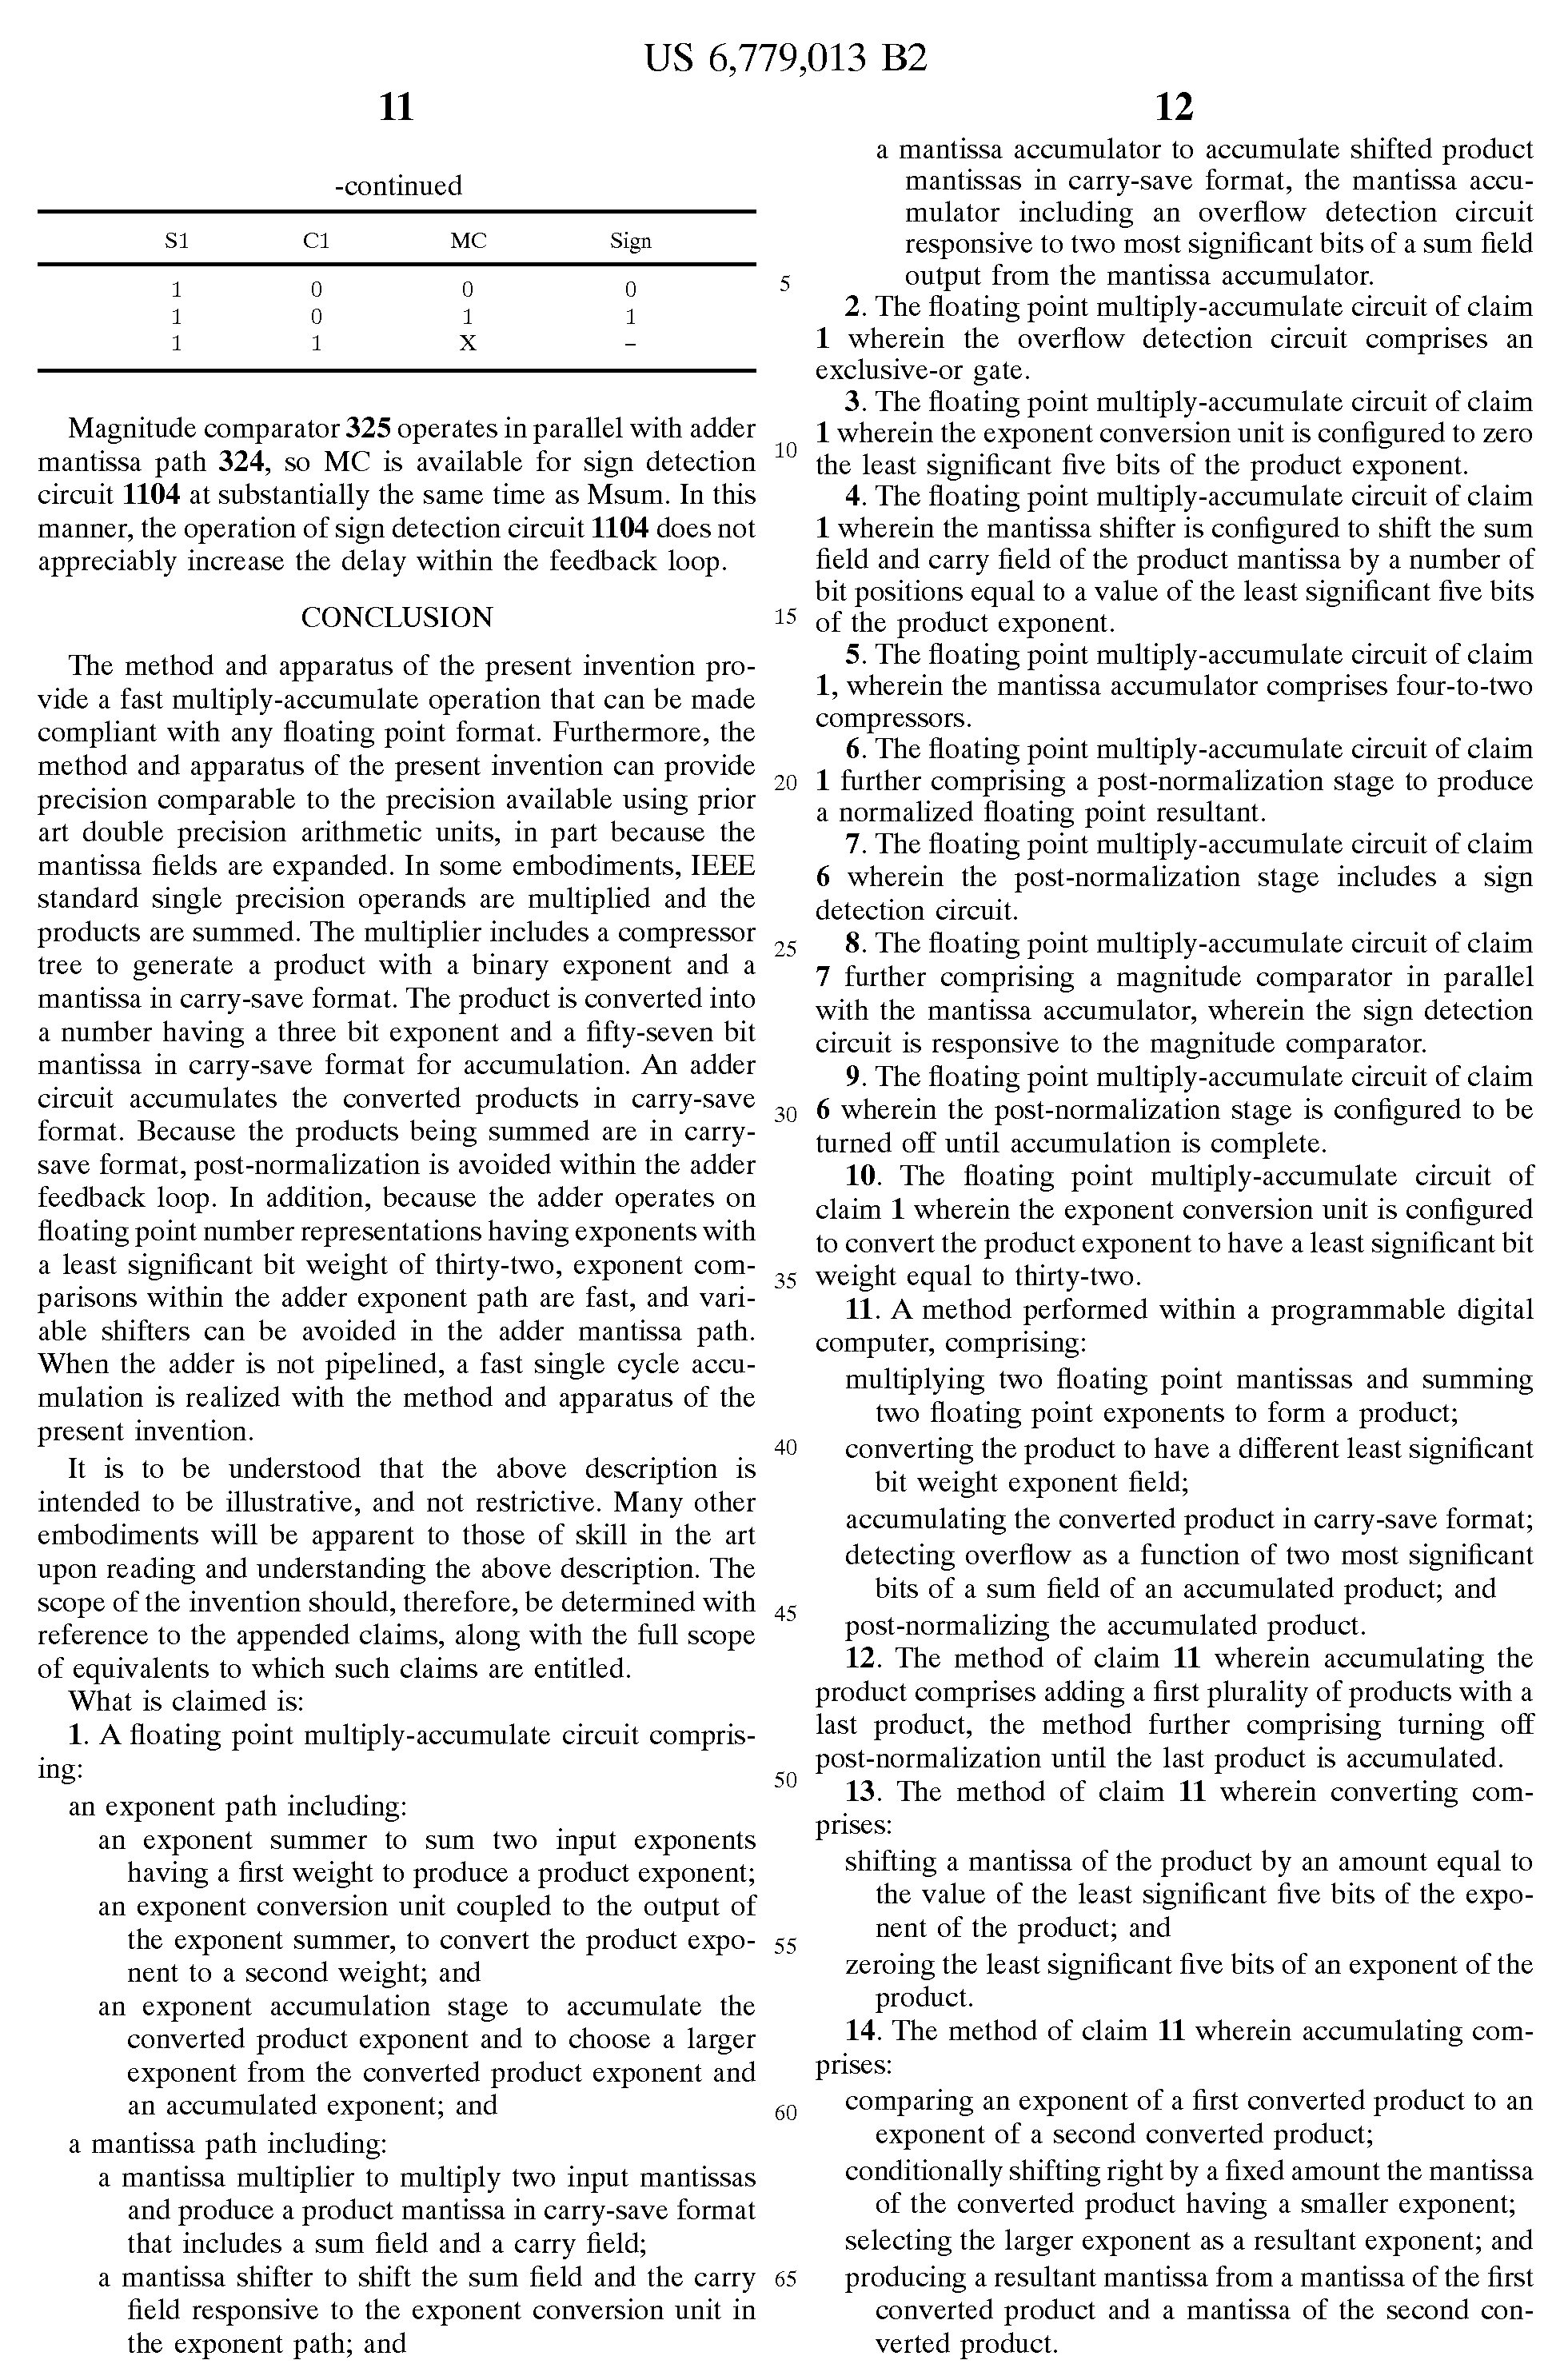
\includegraphics{Fig/media/image3.wmf}. (1)

\textbf{Table B.1} A decision matrix.

\begin{longtable}[]{@{}
  >{\raggedright\arraybackslash}p{(\columnwidth - 10\tabcolsep) * \real{0.1377}}
  >{\raggedright\arraybackslash}p{(\columnwidth - 10\tabcolsep) * \real{0.0975}}
  >{\raggedright\arraybackslash}p{(\columnwidth - 10\tabcolsep) * \real{0.2085}}
  >{\raggedright\arraybackslash}p{(\columnwidth - 10\tabcolsep) * \real{0.2111}}
  >{\raggedright\arraybackslash}p{(\columnwidth - 10\tabcolsep) * \real{0.1341}}
  >{\raggedright\arraybackslash}p{(\columnwidth - 10\tabcolsep) * \real{0.2111}}@{}}
\toprule\noalign{}
\multicolumn{2}{@{}>{\raggedright\arraybackslash}p{(\columnwidth - 10\tabcolsep) * \real{0.2352} + 2\tabcolsep}}{%
\begin{minipage}[b]{\linewidth}\raggedright
\end{minipage}} & \begin{minipage}[b]{\linewidth}\raggedright
\textbf{Alternative 1}
\end{minipage} & \begin{minipage}[b]{\linewidth}\raggedright
\textbf{Alternative 2}
\end{minipage} & \begin{minipage}[b]{\linewidth}\raggedright
\end{minipage} & \begin{minipage}[b]{\linewidth}\raggedright
\textbf{Alternative n}
\end{minipage} \\
\midrule\noalign{}
\endhead
\bottomrule\noalign{}
\endlastfoot
\textbf{Criteria 1} & 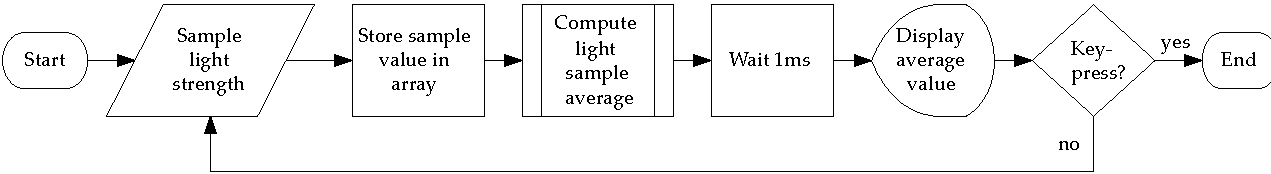
\includegraphics{Fig/media/image4.wmf} &
\emph{α\textsubscript{11}} & \emph{α\textsubscript{12}} &
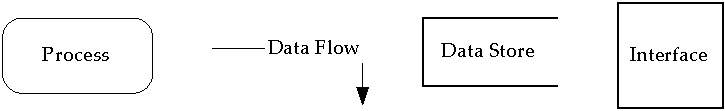
\includegraphics{Fig/media/image5.wmf} & \emph{α\textsubscript{1n}} \\
\textbf{Criteria 2} & 
\includegraphics{Fig/media/image6.wmf} &
\emph{α\textsubscript{21}} & \emph{α\textsubscript{22}} &
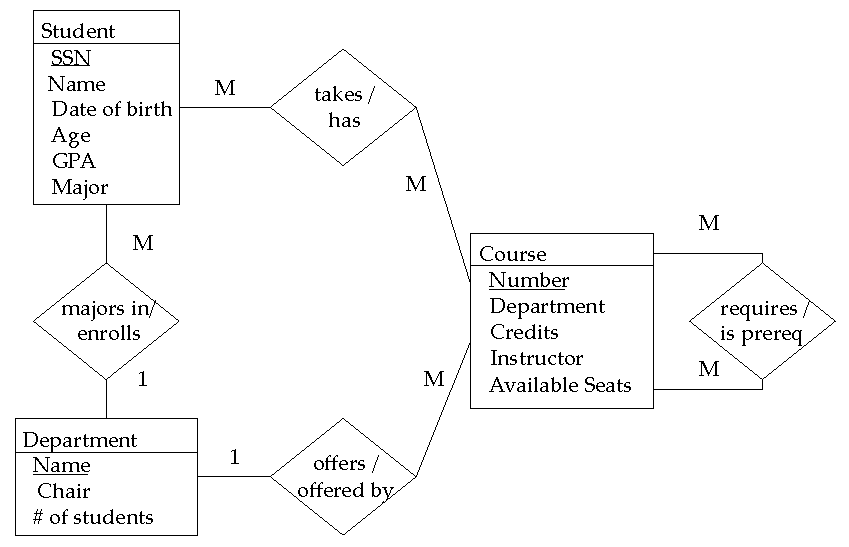
\includegraphics{Fig/media/image7.wmf} & \emph{α\textsubscript{2n}} \\
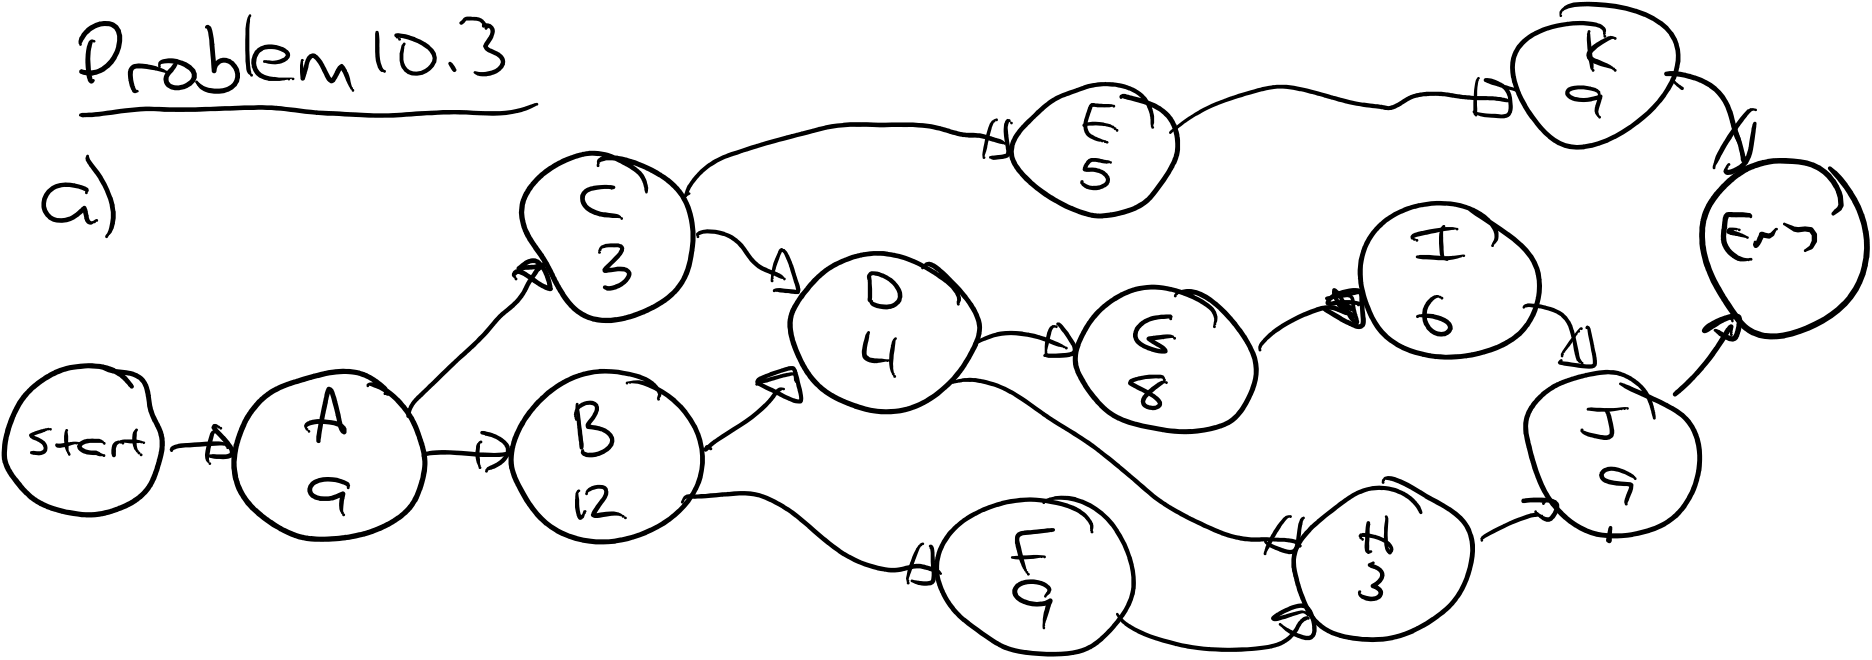
\includegraphics{Fig/media/image8.wmf} &
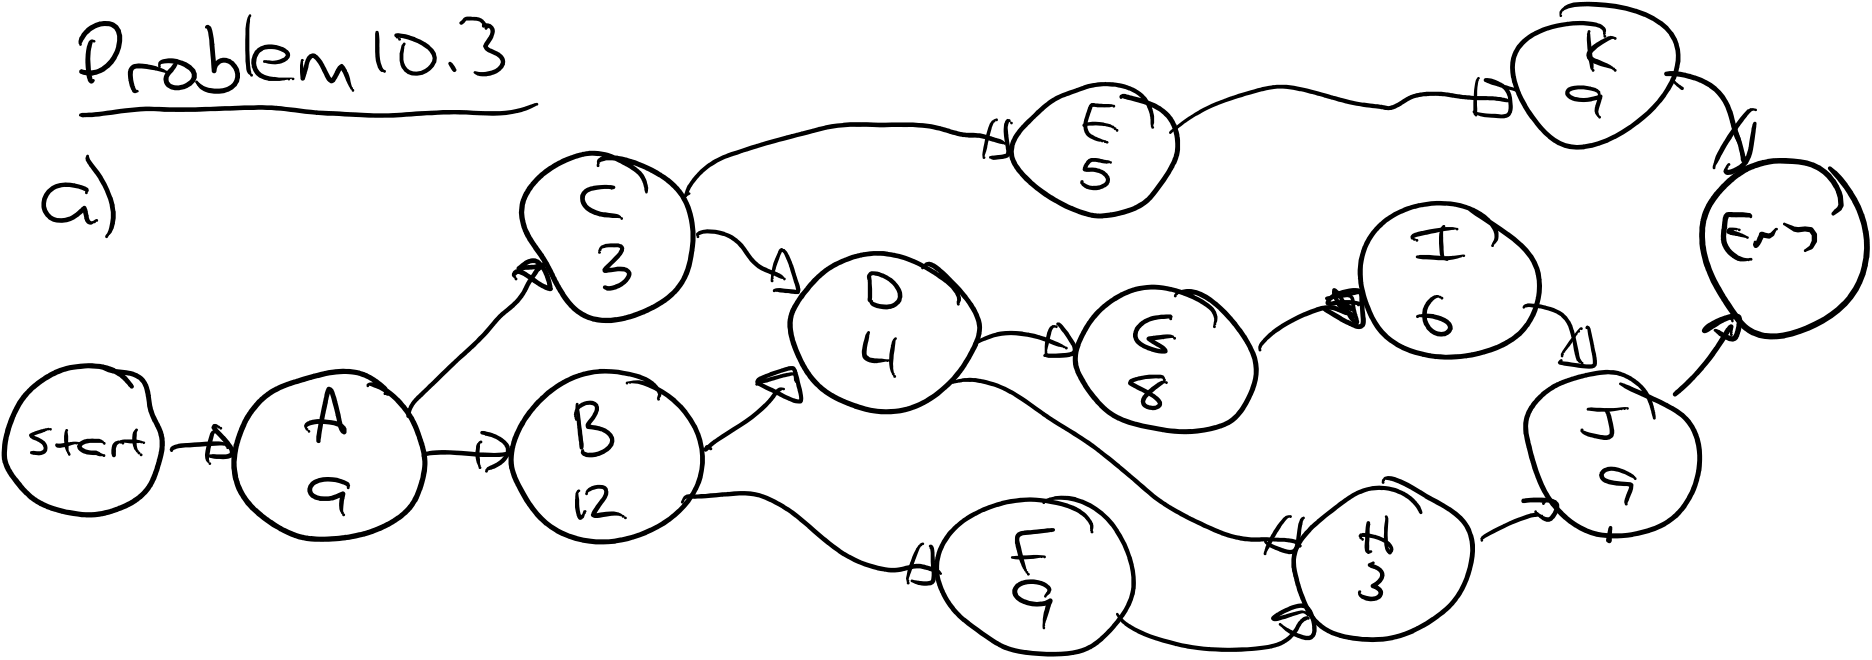
\includegraphics{Fig/media/image8.wmf} &
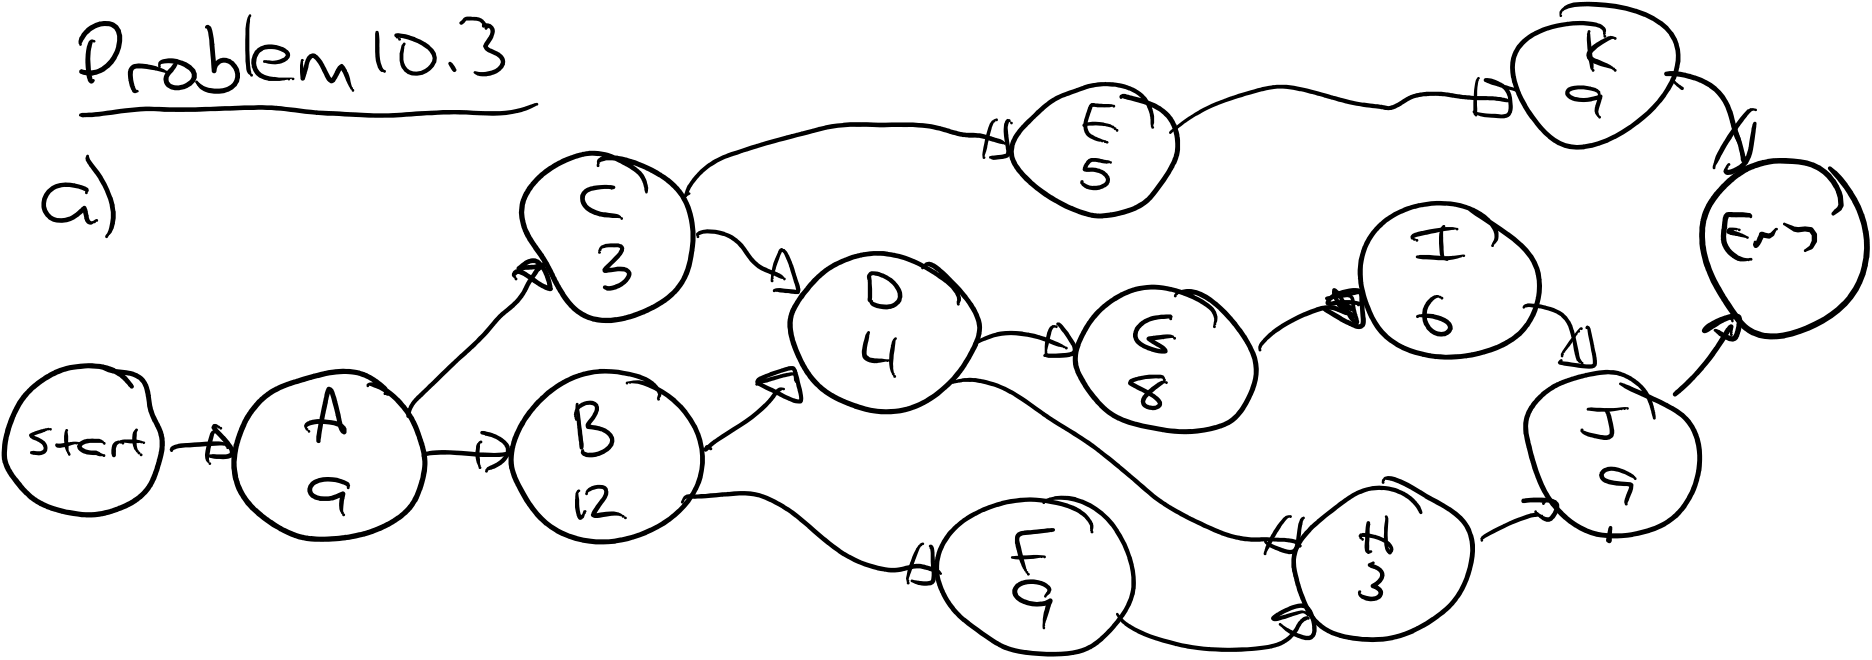
\includegraphics{Fig/media/image8.wmf} &
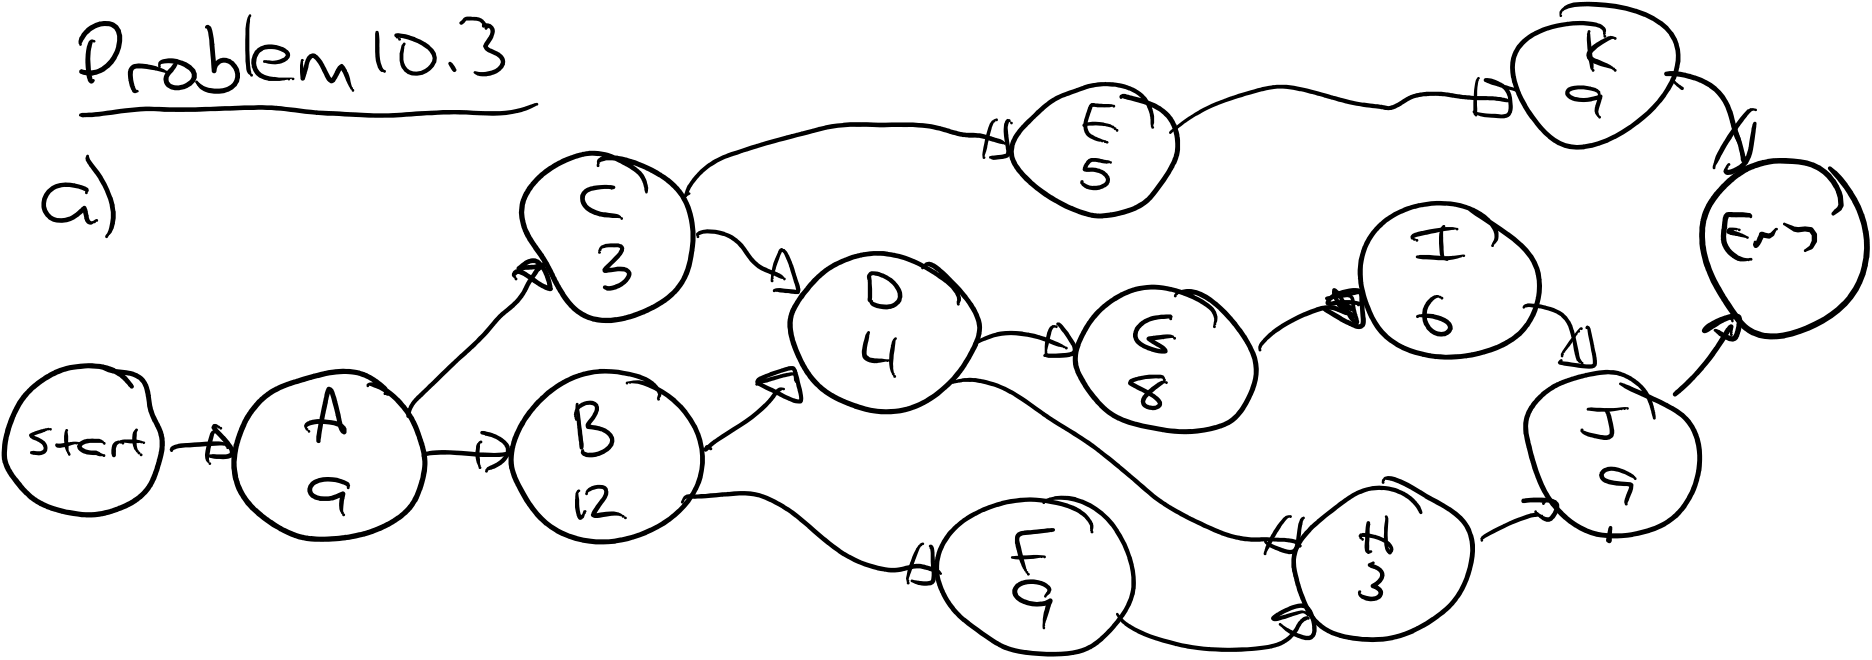
\includegraphics{Fig/media/image8.wmf} &
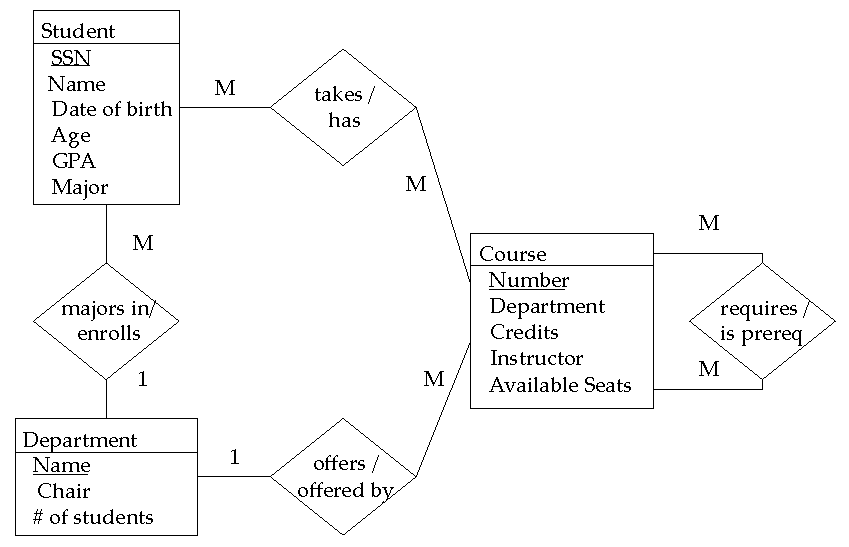
\includegraphics{Fig/media/image7.wmf} &
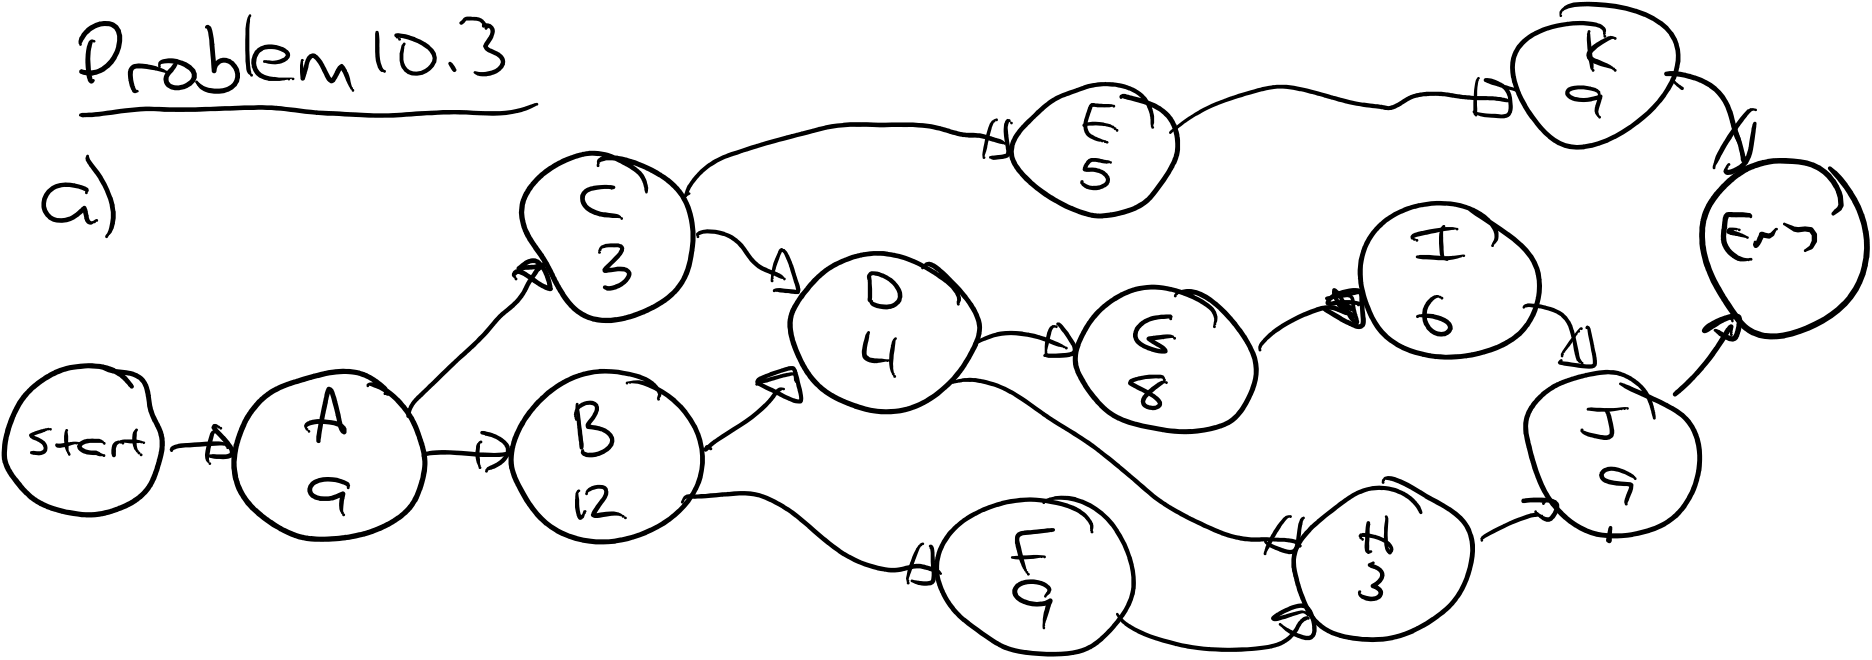
\includegraphics{Fig/media/image8.wmf} \\
\textbf{Criteria \emph{m}} & 
\includegraphics{Fig/media/image9.wmf} &
\emph{α\textsubscript{m1}} & \emph{α\textsubscript{m2}} &
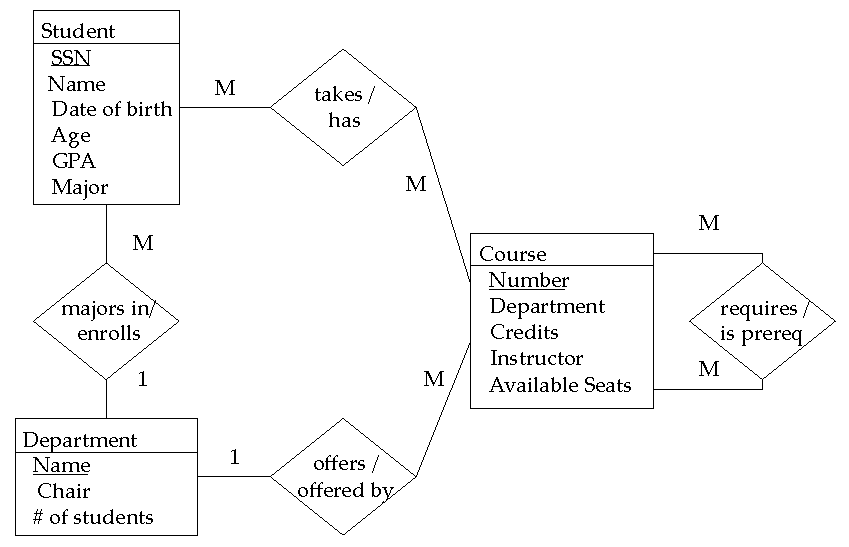
\includegraphics{Fig/media/image7.wmf} & \emph{α\textsubscript{mn}} \\
\multicolumn{2}{@{}>{\raggedright\arraybackslash}p{(\columnwidth - 10\tabcolsep) * \real{0.2352} + 2\tabcolsep}}{%
\textbf{Score}} & 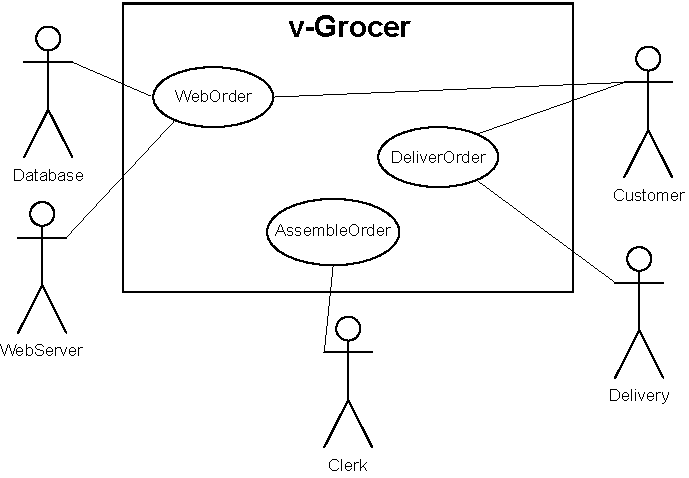
\includegraphics{Fig/media/image10.wmf} &
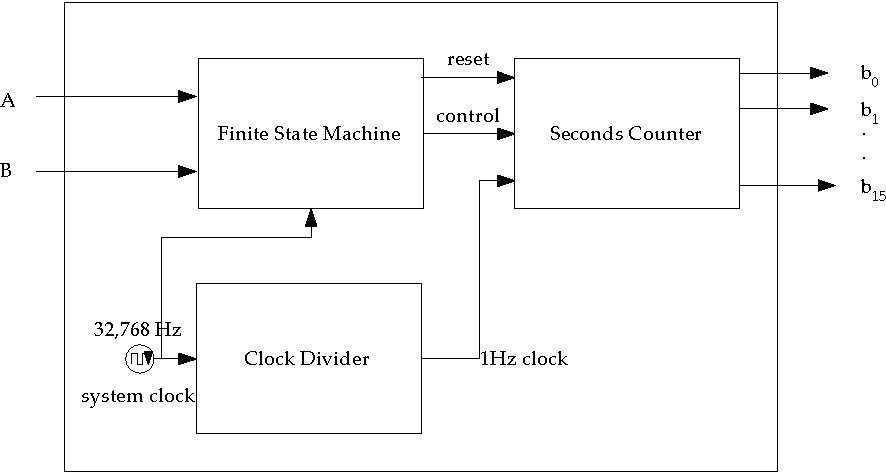
\includegraphics{Fig/media/image11.wmf} &
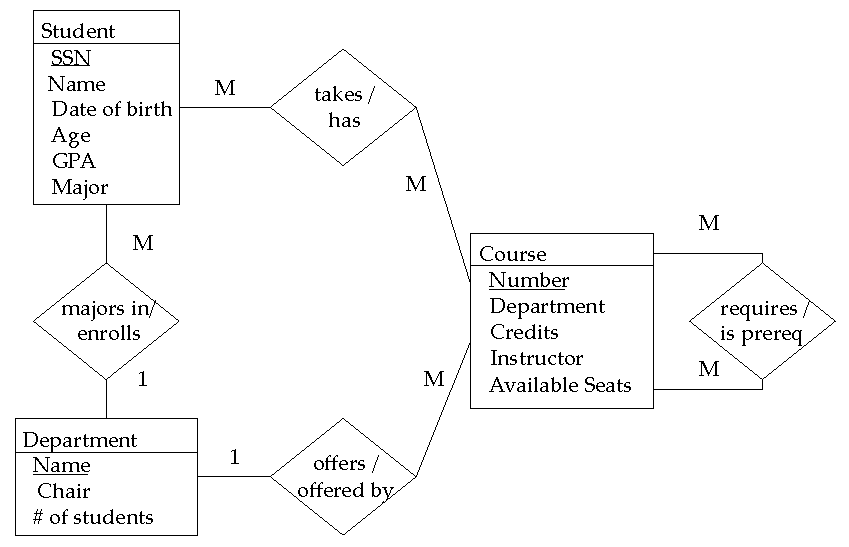
\includegraphics{Fig/media/image7.wmf} &

\includegraphics{Fig/media/image12.wmf} \\
\end{longtable}

The steps of AHP are to:

\begin{enumerate}
\def\labelenumi{\arabic{enumi}.}
\item
  Determine the selection criteria.
\item
  Determine the criteria weightings.
\item
  Identify and rate alternatives relative to the criteria.
\item
  Compute scores for the alternatives.
\item
  Review the decision.
\end{enumerate}

AHP is demonstrated through two examples in which the decision to
purchase a car is considered. This example has the benefit of being
relatively easy to understand, has readily available public data for
supporting the decision, demonstrates the principles of AHP clearly, and
is extensible to design problems. The first example demonstrates a
straightforward set of criteria, while the second extends to
hierarchical criteria.

\subsection{Applying AHP for Car
Selection}\label{applying-ahp-for-car-selection}

AHP is demonstrated in this section by examining the decision to
purchase an automobile.

\subsubsection*{Step 1: Determine the Selection
Criteria}\label{step-1-determine-the-selection-criteria}
\addcontentsline{toc}{subsubsection}{Step 1: Determine the Selection
Criteria}

The first step is to brainstorm to identify the criteria against which
the decision is made -- ideally it is done prior to identification of
the alternatives. The pitfall of identifying alternatives first is that
the criteria may be selected to bias towards a particular alternative.
Assume that the criteria determined are:

\begin{itemize}
\item
  Purchase cost
\item
  Safety
\item
  Design styling
\item
  Brand-name recognition
\end{itemize}

\subsubsection*{Step 2: Determine the Criteria
Weightings}\label{step-2-determine-the-criteria-weightings}
\addcontentsline{toc}{subsubsection}{Step 2: Determine the Criteria
Weightings}

To determine the weights, 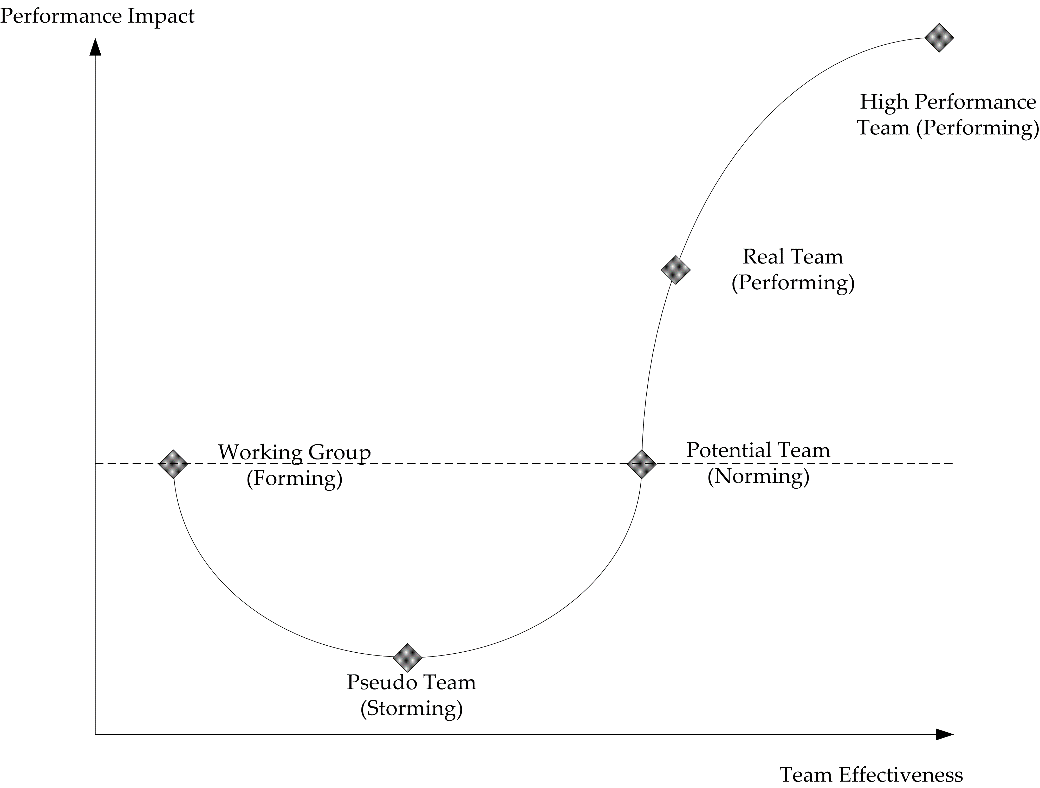
\includegraphics{Fig/media/image1.wmf}\emph{,}
a method known as \emph{\textbf{pairwise comparison}} is applied, where
each criterion is systematically compared to all others. For example,
the purchase cost is compared to safety, design, and brand-name.
Likewise, safety is compared to the remaining criteria and so on. A
common practice in AHP to apply the following scale for pairwise
comparison and it is used throughout the book for consistency

1 = equal, 3 = moderate, 5 = strong, 7 = very strong, 9 = extreme.

For example, if one criterion is deemed strongly more important than
another, it is assigned a score of `5', while if it is deemed strongly
less important, it is assigned the reciprocal value `1/5'.

Example comparisons are captured in the comparison matrix in Table B.2.
For each cell, the corresponding row criterion is compared to the column
criterion. From the first row of the table it is apparent that purchase
cost is considered of equal importance to safety, moderately more
important than design, and very strongly more important than brand-name.
By definition, the diagonal elements are assigned values of 1 since each
is equally important to itself. The matrix should have the following
relationship about the diagonal,

\includegraphics{Fig/media/image13.wmf}.

\textbf{Table B.2} Pairwise comparison of the selection criteria.

\begin{longtable}[]{@{}
  >{\raggedright\arraybackslash}p{(\columnwidth - 8\tabcolsep) * \real{0.2316}}
  >{\raggedright\arraybackslash}p{(\columnwidth - 8\tabcolsep) * \real{0.2079}}
  >{\raggedright\arraybackslash}p{(\columnwidth - 8\tabcolsep) * \real{0.1739}}
  >{\raggedright\arraybackslash}p{(\columnwidth - 8\tabcolsep) * \real{0.1894}}
  >{\raggedright\arraybackslash}p{(\columnwidth - 8\tabcolsep) * \real{0.1973}}@{}}
\toprule\noalign{}
\begin{minipage}[b]{\linewidth}\raggedright
\end{minipage} & \begin{minipage}[b]{\linewidth}\raggedright
\textbf{Purchase cost}
\end{minipage} & \begin{minipage}[b]{\linewidth}\raggedright
\textbf{Safety}
\end{minipage} & \begin{minipage}[b]{\linewidth}\raggedright
\textbf{Design}
\end{minipage} & \begin{minipage}[b]{\linewidth}\raggedright
\textbf{Brand-name}
\end{minipage} \\
\midrule\noalign{}
\endhead
\bottomrule\noalign{}
\endlastfoot
\textbf{Purchase cost} & 1 & 1 & 3 & 7 \\
\textbf{Safety} & 1 & 1 & 5 & 9 \\
\textbf{Design} & 1/3 & 1/5 & 1 & 3 \\
\textbf{Brand-name} & 1/7 & 1/9 & 1/3 & 1 \\
\end{longtable}

People often make comparisons that are inconsistent. Look at the first
row -- purchase cost and safety are deemed to be equally important,
while cost is moderately more important than design (factor of 3). Yet,
in the second row safety is seen as strongly more important than design
(by a factor of 5). This is inconsistent, since if we are to believe the
first row, then safety would be only moderately more important than
design (by a factor of 3) -- just as the purchase cost was compared
relative to safety in the first row.

An intuitive approach for computing the weight for each criterion is to
sum each row. Since a given row represents the comparison of a single
criterion to all others -- the larger a row sum is the more important it
is and the higher the weight it achieves. However, the problem of
inconsistency needs to be addressed. There are a number of approaches
that can be shown mathematically to reduce the inconsistency in the
matrix. A simple method is to take the geometric mean of each row. The
geometric mean of a series of numbers,
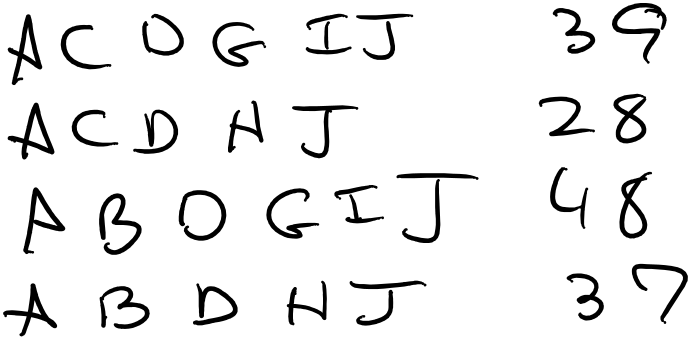
\includegraphics{Fig/media/image14.wmf}, is computed as

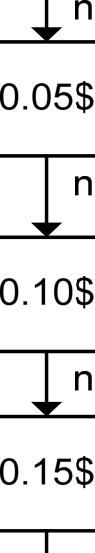
\includegraphics{Fig/media/image15.wmf}. (2)

The geometric mean is often used to reduce bias in skewed data. Table
B.3 demonstrates how the weights are computed. First, the geometric mean
of each row is computed and then the sum of the geometric means is
found. The mean values are divided by the sum to produce a normalized
set of weights (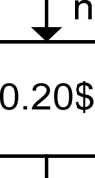
\includegraphics{Fig/media/image16.wmf}). No matter what
method is applied to find the weights, they should be normalized to a
sum of one.

\textbf{Table B.3} Weight values computed from the pairwise comparison.

\begin{longtable}[]{@{}
  >{\raggedright\arraybackslash}p{(\columnwidth - 12\tabcolsep) * \real{0.2000}}
  >{\raggedright\arraybackslash}p{(\columnwidth - 12\tabcolsep) * \real{0.1429}}
  >{\raggedright\arraybackslash}p{(\columnwidth - 12\tabcolsep) * \real{0.1278}}
  >{\raggedright\arraybackslash}p{(\columnwidth - 12\tabcolsep) * \real{0.1217}}
  >{\raggedright\arraybackslash}p{(\columnwidth - 12\tabcolsep) * \real{0.1199}}
  >{\raggedright\arraybackslash}p{(\columnwidth - 12\tabcolsep) * \real{0.1478}}
  >{\raggedright\arraybackslash}p{(\columnwidth - 12\tabcolsep) * \real{0.1400}}@{}}
\toprule\noalign{}
\begin{minipage}[b]{\linewidth}\raggedright
\end{minipage} & \begin{minipage}[b]{\linewidth}\raggedright
\textbf{Purchase cost}
\end{minipage} & \begin{minipage}[b]{\linewidth}\raggedright
\textbf{Safety}
\end{minipage} & \begin{minipage}[b]{\linewidth}\raggedright
\textbf{Design}
\end{minipage} & \begin{minipage}[b]{\linewidth}\raggedright
\textbf{Brand-name}
\end{minipage} & \begin{minipage}[b]{\linewidth}\raggedright
\textbf{Geometric}

\textbf{Mean}
\end{minipage} & \begin{minipage}[b]{\linewidth}\raggedright
\textbf{Weights}
\end{minipage} \\
\midrule\noalign{}
\endhead
\bottomrule\noalign{}
\endlastfoot
\textbf{Purchase cost} & \begin{minipage}[t]{\linewidth}\raggedright
\begin{quote}
1
\end{quote}
\end{minipage} & \begin{minipage}[t]{\linewidth}\raggedright
\begin{quote}
1
\end{quote}
\end{minipage} & \begin{minipage}[t]{\linewidth}\raggedright
\begin{quote}
3
\end{quote}
\end{minipage} & \begin{minipage}[t]{\linewidth}\raggedright
\begin{quote}
7
\end{quote}
\end{minipage} & 2.1 & 0.37 \\
\textbf{Safety} & \begin{minipage}[t]{\linewidth}\raggedright
\begin{quote}
1
\end{quote}
\end{minipage} & \begin{minipage}[t]{\linewidth}\raggedright
\begin{quote}
1
\end{quote}
\end{minipage} & \begin{minipage}[t]{\linewidth}\raggedright
\begin{quote}
5
\end{quote}
\end{minipage} & \begin{minipage}[t]{\linewidth}\raggedright
\begin{quote}
9
\end{quote}
\end{minipage} & 2.6 & 0.46 \\
\textbf{Design} & \begin{minipage}[t]{\linewidth}\raggedright
\begin{quote}
1/3
\end{quote}
\end{minipage} & \begin{minipage}[t]{\linewidth}\raggedright
\begin{quote}
1/5
\end{quote}
\end{minipage} & \begin{minipage}[t]{\linewidth}\raggedright
\begin{quote}
1
\end{quote}
\end{minipage} & \begin{minipage}[t]{\linewidth}\raggedright
\begin{quote}
3
\end{quote}
\end{minipage} & 0.7 & 0.12 \\
\textbf{Brand-name} & \begin{minipage}[t]{\linewidth}\raggedright
\begin{quote}
1/7
\end{quote}
\end{minipage} & \begin{minipage}[t]{\linewidth}\raggedright
\begin{quote}
1/9
\end{quote}
\end{minipage} & \begin{minipage}[t]{\linewidth}\raggedright
\begin{quote}
1/3
\end{quote}
\end{minipage} & \begin{minipage}[t]{\linewidth}\raggedright
\begin{quote}
1
\end{quote}
\end{minipage} & 0.3 & 0.05 \\
\end{longtable}

The criteria have the following weights

\includegraphics{Fig/media/image17.wmf}=0.37,
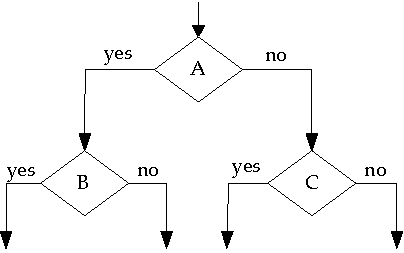
\includegraphics{Fig/media/image18.wmf}=0.46,

\includegraphics{Fig/media/image19.wmf}=0.12, and
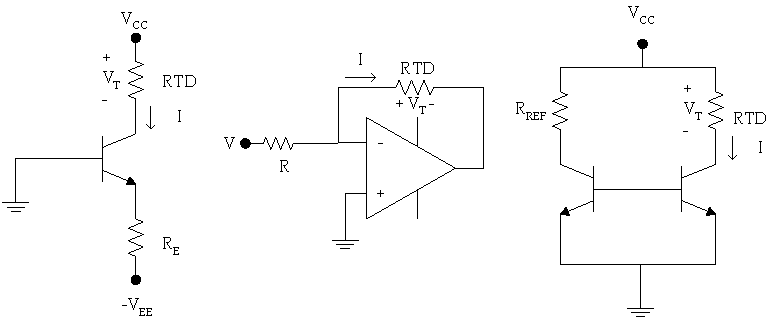
\includegraphics{Fig/media/image20.wmf}=0.05. These calculations are
easily automated with spreadsheet software.

\subsubsection*{Step 3: Identify and Rate Alternatives Relative to the
Criteria}\label{step-3-identify-and-rate-alternatives-relative-to-the-criteria}
\addcontentsline{toc}{subsubsection}{Step 3: Identify and Rate
Alternatives Relative to the Criteria}

The three competing alternatives to be evaluated are the 2006 model year
Honda CR-V, Hyundai Tucson, and Toyota RAV4, which are all small
sport-utility vehicles. The ratings of each alternative relative to each
criterion, 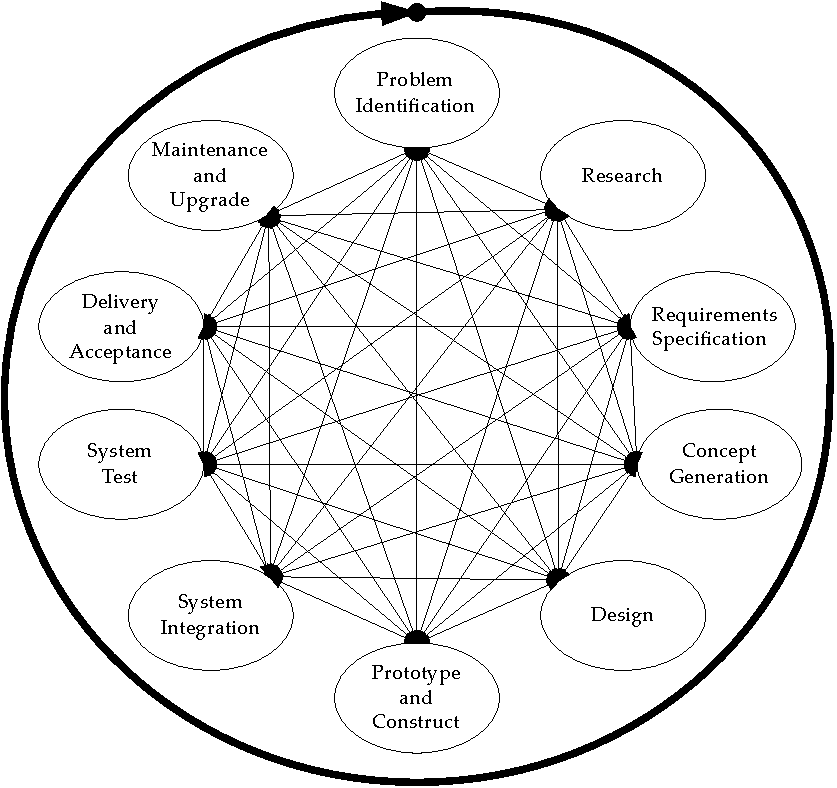
\includegraphics{Fig/media/image2.wmf}, that make up the body
of the decision matrix are determined next. Ideally, quantitative
ratings are determined, but in many cases it is necessary to use a more
qualitative approach. Higher ratings should reflect a better match to
the criteria. Creativity and ingenuity are often needed to determine a
proper metric.

Let's examine purchase cost. The vehicle costs are \$21,026 (Honda),
\$18,183 (Hyundai), and \$21,989 (Toyota). The purchase cost itself
cannot be used directly for a rating metric, since the highest cost
would achieve the highest rating, whereas the objective is to minimize
cost and reward the lowest cost with the highest rating. An alternative
metric is needed. A metric that works when the objective is to minimize
a criterion is to compare it to the minimum of all values using the
following ratio


\includegraphics{Fig/media/image21.wmf}. (3)

This assigns a maximum value of 1 to the lowest cost option, which in
this case is the Hyundai. The cost ratings are computed to be

\includegraphics{Fig/media/image22.wmf}= 0.86,
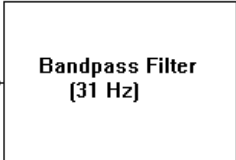
\includegraphics{Fig/media/image23.wmf}= 1, and

\includegraphics{Fig/media/image24.wmf}= 0.83. It is important that the
ratings relative to each criteria be normalized so that their sum is
one. If not, the sum of ratings for each criterion will be different.
This would introduce bias by altering the relative weights of the
criteria. The normalized ratings are

\includegraphics{Fig/media/image22.wmf}= 0.32,
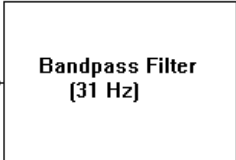
\includegraphics{Fig/media/image23.wmf}= 0.37, and

\includegraphics{Fig/media/image24.wmf}= 0.31.

Next, a metric for safety is needed. Fortunately, there is real data to
draw upon from the US National Highway Transportation Safety Association
(\href{http://www.safercar.gov}{www.safercar.gov}) which rates vehicles
in multiple categories on a five-point scale. The average rating for
each car is 
\includegraphics{Fig/media/image25.wmf}= 4.8 (Honda),

\includegraphics{Fig/media/image26.wmf}=4.8 (Hyundai), and

\includegraphics{Fig/media/image27.wmf}= 4.6 (Toyota), producing the
following normalized values 
\includegraphics{Fig/media/image28.wmf}=
0.34, 
\includegraphics{Fig/media/image29.wmf}= 0.34, and

\includegraphics{Fig/media/image30.wmf}= 0.32.

The rating of the cars relative to the design styling criterion is
considered next. This requires a more subjective approach than the
previous two criteria. To quantify the subjective evaluation pairwise
comparison is again applied to determine the relative value of one
automobile's design to another. Pairwise comparison for the design
styling criteria is shown in Table B.4. The 2006 CR-V is has older
styling, resulting in a much lower design styling rating than the
others.

\textbf{Table B.4} Pairwise comparison of design styling to determine
ratings.

\begin{longtable}[]{@{}
  >{\raggedright\arraybackslash}p{(\columnwidth - 8\tabcolsep) * \real{0.2716}}
  >{\raggedright\arraybackslash}p{(\columnwidth - 8\tabcolsep) * \real{0.1764}}
  >{\raggedright\arraybackslash}p{(\columnwidth - 8\tabcolsep) * \real{0.1842}}
  >{\raggedright\arraybackslash}p{(\columnwidth - 8\tabcolsep) * \real{0.1728}}
  >{\raggedright\arraybackslash}p{(\columnwidth - 8\tabcolsep) * \real{0.1950}}@{}}
\toprule\noalign{}
\begin{minipage}[b]{\linewidth}\raggedright
\end{minipage} & \begin{minipage}[b]{\linewidth}\raggedright
Honda CRV
\end{minipage} & \begin{minipage}[b]{\linewidth}\raggedright
Hyundai

Tucson
\end{minipage} & \begin{minipage}[b]{\linewidth}\raggedright
Toyota

RAV4
\end{minipage} & \begin{minipage}[b]{\linewidth}\raggedright
Design Rating
\end{minipage} \\
\midrule\noalign{}
\endhead
\bottomrule\noalign{}
\endlastfoot
Honda CRV & \begin{minipage}[t]{\linewidth}\raggedright
\begin{quote}
1
\end{quote}
\end{minipage} & \begin{minipage}[t]{\linewidth}\raggedright
\begin{quote}
1/3
\end{quote}
\end{minipage} & \begin{minipage}[t]{\linewidth}\raggedright
\begin{quote}
1/5
\end{quote}
\end{minipage} & 0.11 \\
Hyundai Tucson & \begin{minipage}[t]{\linewidth}\raggedright
\begin{quote}
3
\end{quote}
\end{minipage} & \begin{minipage}[t]{\linewidth}\raggedright
\begin{quote}
1
\end{quote}
\end{minipage} & \begin{minipage}[t]{\linewidth}\raggedright
\begin{quote}
½
\end{quote}
\end{minipage} & 0.31 \\
Toyota RAV4 & \begin{minipage}[t]{\linewidth}\raggedright
\begin{quote}
5
\end{quote}
\end{minipage} & \begin{minipage}[t]{\linewidth}\raggedright
\begin{quote}
2
\end{quote}
\end{minipage} & \begin{minipage}[t]{\linewidth}\raggedright
\begin{quote}
1
\end{quote}
\end{minipage} & 0.58 \\
\end{longtable}

Finally, the ratings for brand-name recognition are determined using
pairwise comparison as shown in Table B.5.

\textbf{Table B.5} Pairwise comparison of brand-name to determine
ratings.

\begin{longtable}[]{@{}
  >{\raggedright\arraybackslash}p{(\columnwidth - 8\tabcolsep) * \real{0.2836}}
  >{\raggedright\arraybackslash}p{(\columnwidth - 8\tabcolsep) * \real{0.1762}}
  >{\raggedright\arraybackslash}p{(\columnwidth - 8\tabcolsep) * \real{0.1673}}
  >{\raggedright\arraybackslash}p{(\columnwidth - 8\tabcolsep) * \real{0.1620}}
  >{\raggedright\arraybackslash}p{(\columnwidth - 8\tabcolsep) * \real{0.2110}}@{}}
\toprule\noalign{}
\begin{minipage}[b]{\linewidth}\raggedright
\end{minipage} & \begin{minipage}[b]{\linewidth}\raggedright
\textbf{Honda}

\textbf{CRV}
\end{minipage} & \begin{minipage}[b]{\linewidth}\raggedright
\textbf{Hyundai Tucson}
\end{minipage} & \begin{minipage}[b]{\linewidth}\raggedright
\textbf{Toyota}

\textbf{RAV4}
\end{minipage} & \begin{minipage}[b]{\linewidth}\raggedright
\textbf{Brand-name rating}
\end{minipage} \\
\midrule\noalign{}
\endhead
\bottomrule\noalign{}
\endlastfoot
\textbf{Honda CRV} & \begin{minipage}[t]{\linewidth}\raggedright
\begin{quote}
1
\end{quote}
\end{minipage} & \begin{minipage}[t]{\linewidth}\raggedright
\begin{quote}
4
\end{quote}
\end{minipage} & \begin{minipage}[t]{\linewidth}\raggedright
\begin{quote}
1
\end{quote}
\end{minipage} & 0.44 \\
\textbf{Hyundai Tucson} & \begin{minipage}[t]{\linewidth}\raggedright
\begin{quote}
¼
\end{quote}
\end{minipage} & \begin{minipage}[t]{\linewidth}\raggedright
\begin{quote}
1
\end{quote}
\end{minipage} & \begin{minipage}[t]{\linewidth}\raggedright
\begin{quote}
¼
\end{quote}
\end{minipage} & 0.12 \\
\textbf{Toyota RAV4} & \begin{minipage}[t]{\linewidth}\raggedright
\begin{quote}
1
\end{quote}
\end{minipage} & \begin{minipage}[t]{\linewidth}\raggedright
\begin{quote}
4
\end{quote}
\end{minipage} & \begin{minipage}[t]{\linewidth}\raggedright
\begin{quote}
1
\end{quote}
\end{minipage} & 0.44 \\
\end{longtable}

Note that the pairwise comparison method can be somewhat time-consuming
since many comparisons must be made. When making subjective estimates, a
faster approach is to use scoring rubric that reflects how well each of
the alternatives meet the criterion, for example

1 = does not meet criterion, 5 = partially meets criterion, 9 =
completely meets criterion.

Keep in mind that pairwise comparison has the advantage of a systematic
comparison of alternatives and this reduces inconsistency in ratings.

\subsubsection*{Step 4: Compute Scores for the
Alternatives}\label{step-4-compute-scores-for-the-alternatives}
\addcontentsline{toc}{subsubsection}{Step 4: Compute Scores for the
Alternatives}

The decision matrix is built and the overall weighted scores for the
alternatives are computed as shown in Table B.6.

\textbf{Table B.6} The decision matrix.

\begin{longtable}[]{@{}
  >{\raggedright\arraybackslash}p{(\columnwidth - 8\tabcolsep) * \real{0.2276}}
  >{\raggedright\arraybackslash}p{(\columnwidth - 8\tabcolsep) * \real{0.1099}}
  >{\raggedright\arraybackslash}p{(\columnwidth - 8\tabcolsep) * \real{0.2212}}
  >{\raggedright\arraybackslash}p{(\columnwidth - 8\tabcolsep) * \real{0.2240}}
  >{\raggedright\arraybackslash}p{(\columnwidth - 8\tabcolsep) * \real{0.2173}}@{}}
\toprule\noalign{}
\multicolumn{2}{@{}>{\raggedright\arraybackslash}p{(\columnwidth - 8\tabcolsep) * \real{0.3375} + 2\tabcolsep}}{%
\begin{minipage}[b]{\linewidth}\raggedright
\end{minipage}} & \begin{minipage}[b]{\linewidth}\raggedright
\textbf{Honda CR-V}
\end{minipage} & \begin{minipage}[b]{\linewidth}\raggedright
\textbf{Hyundai Tucson}
\end{minipage} & \begin{minipage}[b]{\linewidth}\raggedright
\textbf{Toyota RAV4}
\end{minipage} \\
\midrule\noalign{}
\endhead
\bottomrule\noalign{}
\endlastfoot
\textbf{Cost} & 0.37 & 0.32 & 0.37 & 0.31 \\
\textbf{Safety} & 0.46 & 0.34 & 0.34 & 0.32 \\
\textbf{Design styling} & 0.12 & 0.11 & 0.31 & 0.58 \\
\textbf{Brand-name} & 0.05 & 0.44 & 0.12 & 0.44 \\
\multicolumn{2}{@{}>{\raggedright\arraybackslash}p{(\columnwidth - 8\tabcolsep) * \real{0.3375} + 2\tabcolsep}}{%
\textbf{Score}} & \textbf{0.31} & \textbf{0.34} & \textbf{0.35} \\
\end{longtable}

\subsubsection*{Step 5: Review the
Decision}\label{step-5-review-the-decision}
\addcontentsline{toc}{subsubsection}{Step 5: Review the Decision}

The result is a set of numerical scores for the alternatives and if all
work is done properly the final scores should sum to one. In this case
there is not much difference between the scores and a simple decision
based upon the maximum value would lead to selection of the RAV4. Since
there is not much of a difference, all three are good choices based upon
the selection criteria. The decision matrix allows the examination of
different scenarios as the weights and ratings can be varied to see how
they affect the overall scores. The RAV4 beats the Tucson primarily due
to styling and brand-name, which are both subjective ratings. This might
warrant re-visiting those ratings to see how they impact the decision.
The RAV4 barely beats out the Tucson, so if cost and safety are truly
more important, the Tucson is a better decision as it beats the RAV4 in
both of those categories.

\subsection{Hierarchical Decision
Criteria}\label{hierarchical-decision-criteria}

The example in the previous section had fairly simple selection criteria
and it arguably missed some important ones, such as the operating costs.
Further, when considering operating cost it becomes apparent that it has
multiple dimensions, or sub-criteria, such as fuel and insurance costs.
Similarly, the design styling criterion can be sub-divided into interior
and exterior design. Thus there is a hierarchy in the criteria, giving
rise to the name Analytical Hierarchy Process. The following extends the
previous example to include the use of hierarchical criteria.

\subsubsection*{Step 1: Determine the Selection
Criteria}\label{step-1-determine-the-selection-criteria-1}
\addcontentsline{toc}{subsubsection}{Step 1: Determine the Selection
Criteria}

Assume that the criteria have been expanded to be more realistic as
shown below:

\begin{itemize}
\item
  Purchase cost
\item
  Operating costs

  \begin{itemize}
  \item
    Fuel
  \item
    Insurance
  \end{itemize}
\item
  Safety
\item
  Design styling

  \begin{itemize}
  \item
    Interior
  \item
    Exterior
  \end{itemize}
\item
  Brand-name recognition
\end{itemize}

\subsubsection*{Step 2: Determine the Criteria
Weightings}\label{step-2-determine-the-criteria-weightings-1}
\addcontentsline{toc}{subsubsection}{Step 2: Determine the Criteria
Weightings}

Pairwise comparison is again used to determine the weights. The
difference now is that this comparison is done at each level in the
hierarchy. First, purchase cost, operating costs, safety, design, and
brand-name recognition are compared. Then fuel and insurance costs are
compared to each other since they are at the same level and grouping in
the hierarchy, as are exterior and interior design. Assume that the
pairwise comparisons produce the following criteria weights:

\begin{itemize}
\item
  Purchase cost (0.33)
\item
  Operating Costs (0.11)

  \begin{itemize}
  \item
    MPG (0.67)
  \item
    Insurance (0.33)
  \end{itemize}
\item
  Safety (0.40)
\item
  Design Styling (0.12)

  \begin{itemize}
  \item
    Interior (0.50)
  \item
    Exterior (0.50)
  \end{itemize}
\item
  Brand-name recognition (0.04)
\end{itemize}

\subsubsection*{Step 3: Identify and Rate Alternatives Relative to the
Criteria}\label{step-3-identify-and-rate-alternatives-relative-to-the-criteria-1}
\addcontentsline{toc}{subsubsection}{Step 3: Identify and Rate
Alternatives Relative to the Criteria}

Utilizing the results from the previous section, it is only necessary to
compute scores relative to the new criteria. Using mileage per gallon as
a metric for ratings fuel costs is straightforward, since the two are
directly proportional. This data is readily available and is 24, 23, and
25 miles per gallon for the CR-V, Tucson, and RAV4 respectively. This
produces normalized ratings of 0.33, 0.32, and 0.35 respectively.

In terms of insurance costs, the National Highway Transportation Safety
Institute publishes the relative average loss per insured vehicle, a
rating that is used by insurance companies to determine insurance costs.
A score of 100 is the industry average -- those exceeding 100 are above
the average and those less than 100 are below it. The publicly available
ratings are 93, 100, and 112 for the CR-V, Tucson, and RAV4
respectively. Again, the objective is to minimize these values so the
metric in equation (3) is used. This produces normalized ratings of
0.36, 0.34, and 0.30 respectively.

Styling is subjective and ratings could be determined using a scoring
rubric or the pairwise comparison method. Assume that this produces the
scores shown in Table B.7.

\subsubsection*{Step 4: Compute Scores for the
Alternatives}\label{step-4-compute-scores-for-the-alternatives-1}
\addcontentsline{toc}{subsubsection}{Step 4: Compute Scores for the
Alternatives}

The decision-matrix shown in Table B.7 reflects the hierarchical
criteria. The scores are computed slightly differently when sub-criteria
are involved. For example, the score for operating costs of the Honda is
computed based upon the two sub-criteria as (0.67x0.33 + 0.33x0.36) =
0.34. The value of 0.34 is then the rating reflected in table for the
operating costs of this vehicle. Then to get the weighted score for
operating costs, this result of 0.33 is multiplied by the weight of
0.11, exactly as in the previous example.

\textbf{Table B.7} The decision matrix.

\begin{longtable}[]{@{}
  >{\raggedright\arraybackslash}p{(\columnwidth - 8\tabcolsep) * \real{0.2231}}
  >{\raggedright\arraybackslash}p{(\columnwidth - 8\tabcolsep) * \real{0.1372}}
  >{\raggedright\arraybackslash}p{(\columnwidth - 8\tabcolsep) * \real{0.2135}}
  >{\raggedright\arraybackslash}p{(\columnwidth - 8\tabcolsep) * \real{0.2162}}
  >{\raggedright\arraybackslash}p{(\columnwidth - 8\tabcolsep) * \real{0.2100}}@{}}
\toprule\noalign{}
\multicolumn{2}{@{}>{\raggedright\arraybackslash}p{(\columnwidth - 8\tabcolsep) * \real{0.3602} + 2\tabcolsep}}{%
\begin{minipage}[b]{\linewidth}\raggedright
\end{minipage}} & \begin{minipage}[b]{\linewidth}\raggedright
\textbf{Honda CR-V}
\end{minipage} & \begin{minipage}[b]{\linewidth}\raggedright
\textbf{Hyundai Tucson}
\end{minipage} & \begin{minipage}[b]{\linewidth}\raggedright
\textbf{Toyota RAV4}
\end{minipage} \\
\midrule\noalign{}
\endhead
\bottomrule\noalign{}
\endlastfoot
\textbf{Purchase Cost} & 0.33 & 0.32 & 0.37 & 0.31 \\
\textbf{Operating Cost} & 0.11 & 0.34 & 0.32 & 0.33 \\
\begin{minipage}[t]{\linewidth}\raggedright
\begin{quote}
Fuel
\end{quote}
\end{minipage} & \begin{minipage}[t]{\linewidth}\raggedright
\begin{quote}
0.67
\end{quote}
\end{minipage} & \begin{minipage}[t]{\linewidth}\raggedright
\begin{quote}
0.33
\end{quote}
\end{minipage} & \begin{minipage}[t]{\linewidth}\raggedright
\begin{quote}
0.32
\end{quote}
\end{minipage} & \begin{minipage}[t]{\linewidth}\raggedright
\begin{quote}
0.35
\end{quote}
\end{minipage} \\
\begin{minipage}[t]{\linewidth}\raggedright
\begin{quote}
Insurance
\end{quote}
\end{minipage} & \begin{minipage}[t]{\linewidth}\raggedright
\begin{quote}
0.33
\end{quote}
\end{minipage} & \begin{minipage}[t]{\linewidth}\raggedright
\begin{quote}
0.36
\end{quote}
\end{minipage} & \begin{minipage}[t]{\linewidth}\raggedright
\begin{quote}
0.34
\end{quote}
\end{minipage} & \begin{minipage}[t]{\linewidth}\raggedright
\begin{quote}
0.30
\end{quote}
\end{minipage} \\
\textbf{Safety} & 0.40 & 0.34 & 0.34 & 0.32 \\
\textbf{Design Styling} & 0.12 & 0.20 & 0.40 & 0.40 \\
\begin{minipage}[t]{\linewidth}\raggedright
\begin{quote}
Interior
\end{quote}
\end{minipage} & \begin{minipage}[t]{\linewidth}\raggedright
\begin{quote}
0.60
\end{quote}
\end{minipage} & \begin{minipage}[t]{\linewidth}\raggedright
\begin{quote}
0.20
\end{quote}
\end{minipage} & \begin{minipage}[t]{\linewidth}\raggedright
\begin{quote}
0.40
\end{quote}
\end{minipage} & \begin{minipage}[t]{\linewidth}\raggedright
\begin{quote}
0.40
\end{quote}
\end{minipage} \\
\begin{minipage}[t]{\linewidth}\raggedright
\begin{quote}
Exterior
\end{quote}
\end{minipage} & \begin{minipage}[t]{\linewidth}\raggedright
\begin{quote}
0.40
\end{quote}
\end{minipage} & \begin{minipage}[t]{\linewidth}\raggedright
\begin{quote}
0.20
\end{quote}
\end{minipage} & \begin{minipage}[t]{\linewidth}\raggedright
\begin{quote}
0.40
\end{quote}
\end{minipage} & \begin{minipage}[t]{\linewidth}\raggedright
\begin{quote}
0.40
\end{quote}
\end{minipage} \\
\textbf{Brand-name} & 0.04 & 0.44 & 0.12 & 0.44 \\
\multicolumn{2}{@{}>{\raggedright\arraybackslash}p{(\columnwidth - 8\tabcolsep) * \real{0.3602} + 2\tabcolsep}}{%
\textbf{Score}} & 0.32 & 0.35 & 0.33 \\
\end{longtable}

\subsubsection*{Step 5: Review the
Decision}\label{step-5-review-the-decision-1}
\addcontentsline{toc}{subsubsection}{Step 5: Review the Decision}

With this expanded set of criteria, there is a shift in the overall
ranking and the Hyundai Tucson edges out the Toyota RAV4. Frankly, all
three are good choices and reflects the highly competitive car market. A
comparison of vehicles across classes, such as sport-utility, mid-size,
and a luxury car would likely results in a much larger differential in
the scoring, based upon the weighted criteria used here.

\subsection{\texorpdfstring{Summary and Further Reading
}{Summary and Further Reading }}\label{summary-and-further-reading}

The Analytical Hierarchy Process is an effective tool for comparing
competing alternatives that integrates both quantitative and qualitative
judgments. In order to compare alternatives, criteria for comparison are
selected and the relative weights of the criteria assigned. In terms of
selecting the criteria and their weightings, remember the following:

\begin{itemize}
\item
  Ideally, the criteria are selected prior to identification of the
  alternatives. This avoids the trap of selecting the criteria to
  support a pre-conceived decision.
\item
  There is no single correct way to compute the criterion weights.
  However, the pairwise comparison approach is well-accepted. It can be
  a bit time-consuming, particularly when a large number of criteria are
  to be compared. If used properly pairwise comparison reduces bias in
  the decision.
\item
  There are alternatives to pairwise comparison. One is to rank the
  criterion from most important to least important and then assign a
  relative weighting based upon the ranking. Another alternative is to
  utilize a rubric using a semi-qualitative scale, as 1= low importance,
  5 = medium importance, and 9 = extremely important.
\item
  Regardless of how the weights are selected, the sum of the weights
  should be normalized to a value of one.
\end{itemize}

Once the criteria and weights are found, ratings for each option
relative to the criteria are determined. When computing the ratings,
remember the following:

\begin{itemize}
\item
  If quantitative data is available it should be used. It is admittedly
  hard to determine for many problems.
\item
  Appropriate metrics need to be used for rating quantitative data.
\item
  If quantitative data is unavailable, qualitative judgments must be
  made and quantified. Again, the pairwise comparison is a good tool for
  quantifying such judgments. Alternatively, a rubric for rating the
  alternatives against the criteria can be used.
\item
  The ratings relative to each criterion need to be normalized so that
  their sum is equal to one.
\end{itemize}

The final result is a decision-matrix and scores for each of the
alternatives. This matrix allows one to see the quantify decisions
allowing a rationale approach to decision-making, minimizing emotional
factors in the decision

AHP was originally developed by Thomas Saaty {[}Sat88{]} and has found
wide acceptance since. There are software packages available, such as
Expert Choice, that allow for rapid comparison of alternatives and
evaluation
